\documentclass{beamer}
\usepackage[utf8]{inputenc}
\usepackage[spanish]{babel}
\usepackage{hyperref}
\usepackage{verbatim}
\usepackage{listings}

\setbeamercovered{invisible}
\usetheme{Frankfurt}
\usefonttheme{serif}

% Configurar los listings (Códigos)
\renewcommand{\lstlistingname}{Código}
\lstset{
	language=C++,               % Lenguaje
	basicstyle=\ttfamily\footnotesize,  % Tipo de fuente
	keywordstyle=\color{blue},  % Color de palabras clave
	stringstyle=\color{red},    % Color de strings
	commentstyle=\color{gray},  % Color de comentarios
	showstringspaces=false,     % No muestrar el _ cuando el string tiene espacios
	breaklines = true,          % Partir las líneas largas
	breakatwhitespace=true,	    % Partir las líneas en un espacio
	numbers=left,				% Numerar las líneas a la izq
	numberstyle=\tiny,			% Poner los números de las líneas pequeños
	numberblanklines=true,      % Numerar las líneas en blanco
	columns=fullflexible,       % No perder el formato al dejar los espacios
	keepspaces=true,   			% Dejar los espacios insertados
	frame=tb,					% Poner el recuadro
}


\title{Semillero de Programación}
\subtitle{Pila, Cola, DFS y BFS}
\author{Ana Echavarría \and Juan Francisco Cardona}

\institute{Universidad EAFIT}
\date{22 de febrero de 2013}

\begin{document}

\begin{frame}
	\titlepage
\end{frame}

\begin{frame}
	\frametitle{Contenido}
	\tableofcontents
\end{frame}

\section{Tarea Semana Anterior}
	\begin{frame}[fragile]
		\frametitle{10055 - Hashmat the Brave Warrior}
		\begin{lstlisting}
			int main(){
			   long long a, b;
			   while(cin >> a >> b){
			      long long diff = abs(b - a);
			      cout << diff << endl;
			   }
			    return 0;
			}
		\end{lstlisting}
	\end{frame}
	
	\begin{frame}[fragile]
		\frametitle{100 - The 3n + 1 problem}
		\begin{lstlisting}
			int main(){
			   int i, j;
			   while(cin >> i >> j){
			      cout << i << " " << j << " ";
			      if (i > j) swap(i, j);
			      int best = 0;
			      for (int k = i; k <= j; k++){
			         int count = 1;
			         int n = k;
			         while (n > 1){
			            if (n % 2 == 0) n /= 2;
			            else n = 3 * n + 1;
			            count++;
			         }
			         best = max(count, best);
			      }
			      cout << best << endl;
			   }   
			   return 0;
			}
		\end{lstlisting}
	\end{frame}
	
	\begin{frame}[fragile]
		\frametitle{573 - The Snail}
		\begin{lstlisting}
			int main(){
			   int H, U, D, F;
			   while (cin >> H >> U >> D >> F){
			      if (H == 0) break;
			      int day = 0;
			      double height = 0.0;
			      double climb = U;
			      double fatigue = (1.0 * U * F) / 100;
			      while (height >= 0){
			         height += climb;
			         day++;
			         if (height > H) break;
			         height -= D;
			         climb = max(0.0, climb - fatigue);
			      }
			      if (height >= H) printf("success on day %d\n", day);
			      else printf("failure on day %d\n", day);
			   }
			    return 0;
			}
		\end{lstlisting}
	\end{frame}
	
	\begin{frame}[fragile]
		\frametitle{483 - Word Scramble}
		\begin{lstlisting}
			vector <string> v;
			int main(){
			   string line;
			   while (getline(cin, line)){
			      stringstream ss(line);
			      v.clear();
			      string s;
			      while (ss >> s) v.push_back(s);

			      for (int i = 0; i < v.size(); ++i){
			         reverse(v[i].begin(), v[i].end());
			         if (i > 0) cout << " ";
			         cout << v[i] << " ";
			      }
			      cout << endl;
			   }
			   return 0;
			}
		\end{lstlisting}
		
	\end{frame}


\section{Pila}
	\begin{frame}
		\frametitle{Pila o Stack}
		\begin{block}{Pila o Stack}
			Es una contenedor dinámico en el cual sólo se pueden insertar elementos al final y sólo se pueden extraer elementos del final.\\
			\textbf{El último elemento que se insertó es el primer elemento en salir (LIFO).}\\
		\end{block}		
		Un ejemplo sería una pila de libros.\\
		\begin{center}
			
\includegraphics[height = 0.35\textheight]{stack_libros.jpg}
		\end{center}
	\end{frame}
	
	\begin{frame}
		\frametitle{Operaciones}
		Sobre una \textbf{pila} se pueden realizar las siguientes operaciones
		\begin{description}
			\item[Push(x)] inserta el elemento x al stack.
			\item[Pop()] elimina el último elemento del stack.
			\item[Top()] retorna el último elemento almacenado.
		\end{description}
	\end{frame}
	
	\begin{frame}[fragile]
		\frametitle{Implementación usando la librería de C++}
		\begin{lstlisting}
			#include <iostream>
			#include <stack>            // Incluir stack
			using namespace std;

			int main(){
			   stack <int> s;            // Crear un stack de enteros
			   s.push(10);               // Insertar 10
			   s.push(-1);               // Insertar -1
			   cout << s.top() << endl;  // Imprimir -1
			   s.pop();                  // Eliminar -1
			   cout << s.top() << endl;  // Imprimir 10
			   cout << s.size() << endl; // El tamano del stack es 1
			   return 0;
			}
		\end{lstlisting}
	\end{frame}
	
\section{Cola}
	\begin{frame}
		\frametitle{Cola o Queue}
		\begin{block}{Cola o Queue}
			Es una contenedor dinámico en el cual sólo se pueden insertar elementos al final y sólo se pueden extraer elementos del principio.\\
			\textbf{El primer elemento que se insertó es el primer elemento en salir (FIFO).}\\
		\end{block}		
		Un ejemplo sería una cola en un banco.\\
		\begin{center}
			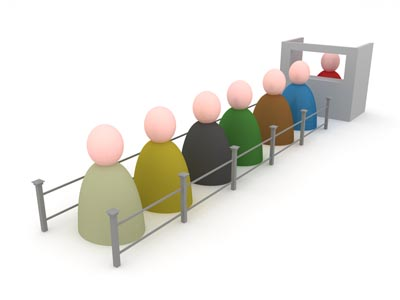
\includegraphics[height = 0.4\textheight]{queue_banco.jpg}
		\end{center}
	\end{frame}
	
	\begin{frame}
		\frametitle{Operaciones}
		Sobre una \textbf{cola} se pueden hacer las siguientes operaciones
		\begin{description}
			\item[Push(x)] inserta el elemento x a la cola.
			\item[Pop()] elimina el primer elemento de la cola.
			\item[Front()] retorna el primer elemento de la cola.
			\item[Back()] retorna el último elemento de la cola
		\end{description}
	\end{frame}
	
	\begin{frame}[fragile]
		\frametitle{Implementación usando la librería de C++}
		\begin{lstlisting}
			#include <iostream>
			#include <queue>               // Incluir queue
			using namespace std;

			int main(){
			   queue <int> q;              // Crear una cola de enteros
			   q.push(10);                 // Insertar 10
			   q.push(-1);                 // Insertar -1
			   cout << q.front() << endl;  // Imprimir 10
			   q.pop();                    // Eliminar 10
			   cout << q.front() << endl;  // Imprimir -1
			   cout << q.size() << endl;   // El tamano de la cola es 1
			   return 0;
			}
		\end{lstlisting}
	\end{frame}
	
\section{BFS: Breadth-First Search}
	\begin{frame}
		\frametitle{BFS}
		\begin{itemize}
			\item Algoritmo para recorrer o buscar elementos en un grafo.
			\item Se comienza desde uno nodo y se exploran todos los vecinos de este nodo.
			\item Luego, para cada uno de los vecinos, se exploran sus respectivos vecinos (que no se hayan visto antes).
			\item Se continúa de esta manera hasta que se haya recorrido todo el grafo.
		\end{itemize}
	\end{frame}
	
	\begin{frame}
		\frametitle{Ejemplos}
		\begin{columns}
			\column{0.4\textwidth}
				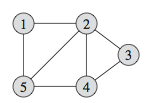
\includegraphics[width = 1.05\textwidth]{GrafoND.png}
			\column{0.5\textwidth}
				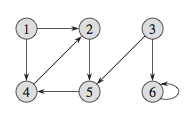
\includegraphics[width = 1.10\textwidth]{GrafoD.png}
		\end{columns}
	\end{frame}
	
	\begin{frame}
		\frametitle{Pregunta}
		\begin{alertblock}{Complejidad}
			\begin{itemize}
				\item ¿Cuántas veces visto cada nodo?
				\item ¿Cuántas veces visito cada arista?
				\item De acuerdo a lo anterior ¿Cuál sería una aproximación a la complejidad del algoritmo?
			\end{itemize}
		\end{alertblock}
		\setbeamercovered{transparent}
		\pause
		\begin{alertblock}{Estructura de datos}
			De las estructuras de datos mostradas anteriormente ¿Cuál sería la apropiada para almacenar los nodos que tengo pendientes por visitar?
		\end{alertblock}
		\setbeamercovered{invisible}
	\end{frame}
	
	\begin{frame}[fragile]
		\frametitle{Algoritmo BFS}
		\begin{lstlisting}
			vector <int> g[MAXN];   // La lista de adyacencia
			int d[MAXN];            // Aristas usadas desde la fuente

			void bfs(int s, int n){ // s = fuente, n = numero de nodos
			   // Marcar todos los nodos como no visitados
			   for (int i = 0; i < n; ++i) d[i] = -1;
			   queue <int> q;                
			   q.push(s);                  // Agregar la fuente a la cola
			   d[s] = 0;                   // La distancia de la fuente es 0
			   while (q.size() > 0){
			      int cur = q.front(); q.pop();
			      for (int i = 0; i < g[cur].size(); ++i){
			         int next = g[cur][i];
			         if (d[next] == -1){       // Si todavía no lo he visitado
			            d[next] = d[cur] + 1;  // La distancia que llevo + 1
			            q.push(next);          // Agregarlo a la cola
			         }
			      }
			   }
			}
		\end{lstlisting}
	\end{frame}
	
	\begin{frame}
		\frametitle{Aplicaciones}
		\begin{itemize}
			\item Buscar o recorrer elementos en un grafo.
			\item Hallar mínimo número de aristas para llegar de la fuente a cualquier nodo.
			\item Hallar los nodos alcanzables desde la fuente (Ver si existe un camino de la fuente a cualquier nodo).
			\item Si se guarda el nodo del que vine (padre), se pueden hallar las aristas pertenecientes al camino ``más corto'' desde la fuente hasta cada nodo.
			\item Con algunas modificaciones sirve para ver si existe un ciclo en algún camino que sale desde la fuente.
		\end{itemize}
	\end{frame}
	
	\begin{frame}
		\frametitle{Complejidad}
		\begin{block}{Complejidad de BFS}
			\begin{itemize}
				\item Si se representa usando la \textbf{lista de adyacencia} la complejidad del BFS es $O(V+E)$.
				\item Si se representa usando la \textbf{matriz de adyacencia} la complejidad del BFS es $O(V^2)$.
			\end{itemize}
		\end{block}
	\end{frame}
	
\section{DFS: Depth-First Search}
	\begin{frame}
		\frametitle{DFS}
		\begin{itemize}
			\item Algoritmo para recorrer o buscar elementos en un grafo.
			\item Se comienza desde uno nodo y se marca como gris (parcialmente visitado).
			\item Se explora cada uno de los vecinos de ese nodo.
			\item Cuando termino de visitar todos los vecinos, marco el nodo como negro (visitado).
			\item En otras palabras, no visito un nodo hasta haber visitado todos sus vecinos.
		\end{itemize}
	\end{frame}
	
	\begin{frame}
		\frametitle{Ejemplos}
		\begin{columns}
			\column{0.4\textwidth}
				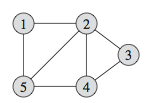
\includegraphics[width = 1.05\textwidth]{GrafoND.png}
			\column{0.5\textwidth}
				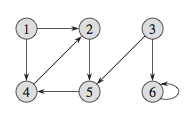
\includegraphics[width = 1.10\textwidth]{GrafoD.png}
		\end{columns}
	\end{frame}
	
	\begin{frame}
		\frametitle{Pregunta}
		\begin{alertblock}{Complejidad}
			\begin{itemize}
				\item ¿Cuántas veces visto cada nodo?
				\item ¿Cuántas veces visito cada arista?
				\item De acuerdo a lo anterior ¿Cuál sería una aproximación a la complejidad del algoritmo?
			\end{itemize}
		\end{alertblock}
		\setbeamercovered{transparent}
		\pause
		\begin{alertblock}{Estructura de datos}
			De las estructuras de datos mostradas anteriormente ¿Cuál sería la apropiada para almacenar los nodos que tengo pendientes por visitar?
		\end{alertblock}
		\setbeamercovered{invisible}
	\end{frame}
	
	\begin{frame}[fragile]
		\frametitle{Algoritmo DFS}
		\begin{lstlisting}
			vector <int> g[MAXN];      // La lista de adyacencia
			int color[MAXN];           // El arreglo de visitados
			enum {WHITE, GRAY, BLACK}; // WHITE = 1, GRAY = 2, BLACK = 3

			void dfs(int u){
			   color[u] = GRAY;   // Marcar el nodo como semi-visitado
			   for (int i = 0; i < g[u].size(); ++i){
			      int v = g[u][i];
			      if (color[v] == WHITE) dfs(v);  // Visitar mis vecinos
			   }
			   color[u] = BLACK;  // Marcar el nodo como visitado
			}

			void call_dfs(int n){
			   // Marcar los nodos como no visitados
			   for (int u = 0; u < n; ++u) color[u] = WHITE;
			   // Llamar la funcion DFS con los nodos no visitados
			   for (int u = 0; u < n; ++u)
			      if (color[u] == WHITE) dfs(u);
			}
		\end{lstlisting}
	\end{frame}
	
	\begin{frame}
		\frametitle{Aplicaciones}
		\begin{itemize}
			\item Buscar o recorrer elementos en un grafo.
			\item Si se guarda el nodo del que vine (padre), se pueden hallar un camino desde la fuente hasta cada nodo.
			\item Ver si existe un ciclo en el grafo (si uno de mis vecinos es gris cuando lo voy a visitar).
			\item Se puede hacer que el DFS retorne algún valor y verificar con él condiciones en el grafo.
			\item Si se modifica el color por el ciclo en el que visité el nodo puedo hallar los nodos alcanzables desde el nodo en el que hago el llamado inicial.
		\end{itemize}
	\end{frame}
	
	\begin{frame}
		\frametitle{Complejidad}
		\begin{block}{Complejidad de DFS}
			\begin{itemize}
				\item Si se representa usando la \textbf{lista de adyacencia} la complejidad del DFS es $O(V+E)$.
				\item Si se representa usando la \textbf{matriz de adyacencia} la complejidad del DFS es $O(V^2)$.
			\end{itemize}
		\end{block}
	\end{frame}

\section{Tarea}
	\begin{frame}
		\frametitle{Tarea}
		\begin{alertblock}{Tarea}
			\begin{itemize}
				\item Resolver los problemas de http://contests.factorcomun.org/contests/50 \\
				\item Para cada problema pensar: ¿Cómo se construiría el grafo? ¿Es dirigido o no dirigido? ¿Debo usar BFS, DFS o cualquiera de las dos?
			\end{itemize}
		\end{alertblock}
	\end{frame}
	
	\begin{frame}
		\frametitle{Ayuda para la tarea}
		\begin{exampleblock}{Ayuda para cada problema}
			\begin{itemize}
				\item[A] El grafo es general para todos los casos de prueba (no cambia). Cuando se vaya a visitar un nodo, verificar que no esté en la lista de los prohibidos.
				\item[B] Si uno de mis vecinos ya está visitado, verificar que su color sea el contrario al mío si no es así retorne falso.
				\item[C] Pensar ¿Cuáles son las fichas que seguro tengo que derribar a mano?. Empujar esas fichas y las que ellas derriben (marcarlas como visitadas). Si luego de esto me quedan fichas sin tumbar ¿Qué característica especial cumplen esas fichas? ¿Cómo las debo derribar?
			\end{itemize}
		\end{exampleblock}
	\end{frame}
	
\end{document}